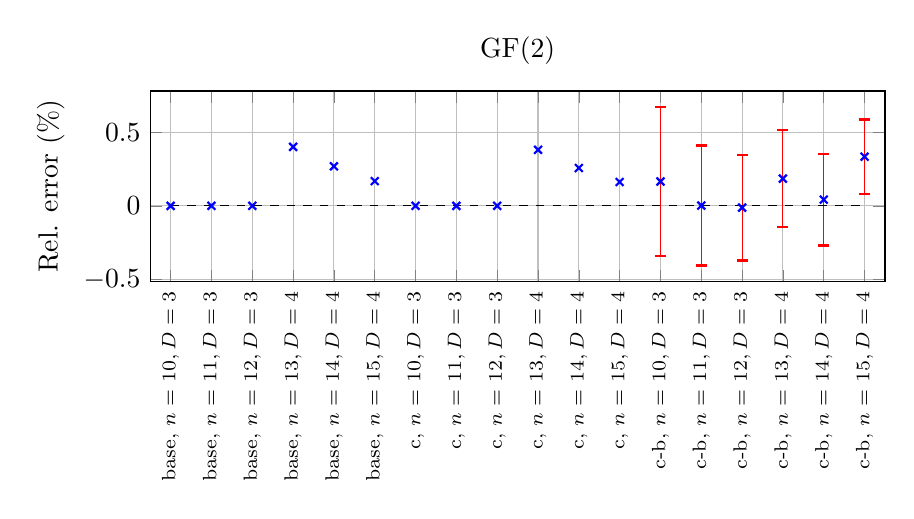
\begin{tikzpicture}
\begin{axis}[
width=0.9\linewidth,
height=0.33\linewidth,
title={$\mathrm{GF}(2)$},
enlarge x limits={abs=0.5},
ylabel={Rel. error (\%)},
xtick=data,
xticklabels={
{base, $n=10, D=3$},{base, $n=11, D=3$},{base, $n=12, D=3$},{base, $n=13, D=4$},{base, $n=14, D=4$},{base, $n=15, D=4$},{c, $n=10, D=3$},{c, $n=11, D=3$},{c, $n=12, D=3$},{c, $n=13, D=4$},{c, $n=14, D=4$},{c, $n=15, D=4$},{c-b, $n=10, D=3$},{c-b, $n=11, D=3$},{c-b, $n=12, D=3$},{c-b, $n=13, D=4$},{c-b, $n=14, D=4$},{c-b, $n=15, D=4$}
},
x tick label style={rotate=90, anchor=east, font=\scriptsize},
grid=both,
]
\addplot+[
only marks,
mark=x,
mark options={line width=0.8pt},
error bars/.cd,
y dir=both,
y explicit,
error bar style={red},
error mark=|,
error mark options={red, line width=0.8pt}
] coordinates {
(1,0.000000)
(2,0.000000)
(3,0.000000)
(4,0.400828)
(5,0.268674)
(6,0.168213)
(7,0.000000)
(8,0.000000)
(9,0.000000)
(10,0.380767)
(11,0.257111)
(12,0.161925)
(13,0.165420) +- (0,0.507683)
(14,0.001672) +- (0,0.408034)
(15,-0.012076) +- (0,0.360311)
(16,0.184958) +- (0,0.330579)
(17,0.042051) +- (0,0.312094)
(18,0.333834) +- (0,0.253229)
};
\addplot[no marks, dashed] coordinates {(1,0) (18,0)};
\end{axis}
\end{tikzpicture}
\par\medskip
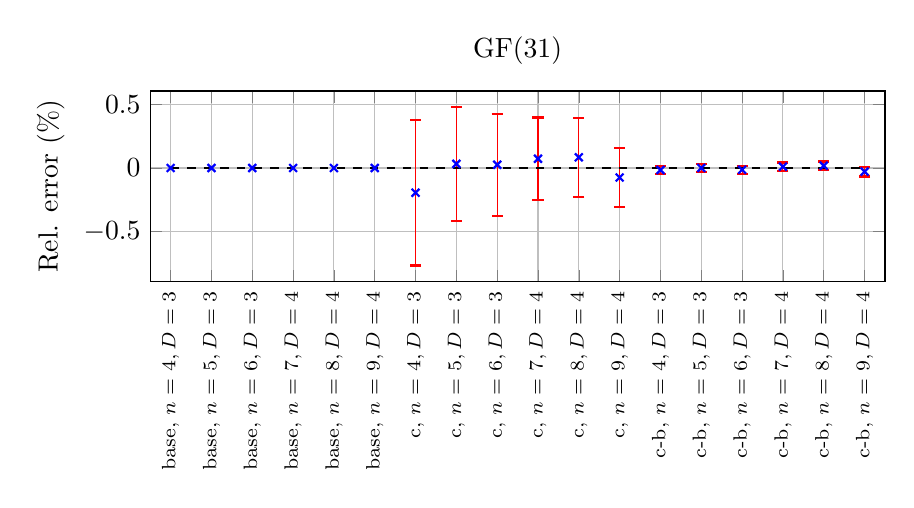
\begin{tikzpicture}
\begin{axis}[
width=0.9\linewidth,
height=0.33\linewidth,
title={$\mathrm{GF}(31)$},
enlarge x limits={abs=0.5},
ylabel={Rel. error (\%)},
xtick=data,
xticklabels={
{base, $n=4, D=3$},{base, $n=5, D=3$},{base, $n=6, D=3$},{base, $n=7, D=4$},{base, $n=8, D=4$},{base, $n=9, D=4$},{c, $n=4, D=3$},{c, $n=5, D=3$},{c, $n=6, D=3$},{c, $n=7, D=4$},{c, $n=8, D=4$},{c, $n=9, D=4$},{c-b, $n=4, D=3$},{c-b, $n=5, D=3$},{c-b, $n=6, D=3$},{c-b, $n=7, D=4$},{c-b, $n=8, D=4$},{c-b, $n=9, D=4$}
},
x tick label style={rotate=90, anchor=east, font=\scriptsize},
grid=both,
]
\addplot+[
only marks,
mark=x,
mark options={line width=0.8pt},
error bars/.cd,
y dir=both,
y explicit,
error bar style={red},
error mark=|,
error mark options={red, line width=0.8pt}
] coordinates {
(1,0.000000)
(2,0.000000)
(3,0.000000)
(4,0.000000)
(5,0.000000)
(6,0.000000)
(7,-0.194622) +- (0,0.573440)
(8,0.032403) +- (0,0.449091)
(9,0.025646) +- (0,0.400480)
(10,0.073020) +- (0,0.324193)
(11,0.084452) +- (0,0.311851)
(12,-0.074793) +- (0,0.232552)
(13,-0.015571) +- (0,0.029297)
(14,0.000421) +- (0,0.030707)
(15,-0.013750) +- (0,0.031828)
(16,0.010631) +- (0,0.033470)
(17,0.018080) +- (0,0.032379)
(18,-0.028424) +- (0,0.038421)
};
\addplot[no marks, dashed] coordinates {(1,0) (18,0)};
\end{axis}
\end{tikzpicture}
\par\medskip
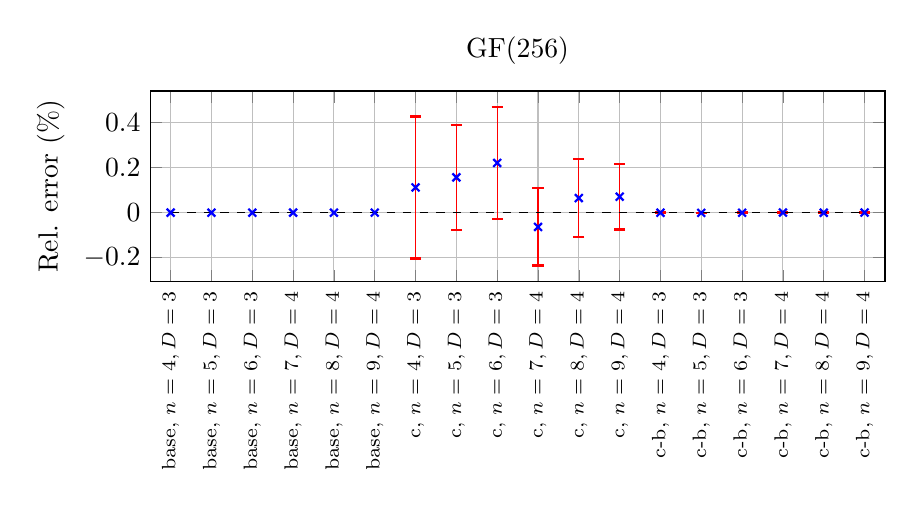
\begin{tikzpicture}
\begin{axis}[
width=0.9\linewidth,
height=0.33\linewidth,
title={$\mathrm{GF}(256)$},
enlarge x limits={abs=0.5},
ylabel={Rel. error (\%)},
xtick=data,
xticklabels={
{base, $n=4, D=3$},{base, $n=5, D=3$},{base, $n=6, D=3$},{base, $n=7, D=4$},{base, $n=8, D=4$},{base, $n=9, D=4$},{c, $n=4, D=3$},{c, $n=5, D=3$},{c, $n=6, D=3$},{c, $n=7, D=4$},{c, $n=8, D=4$},{c, $n=9, D=4$},{c-b, $n=4, D=3$},{c-b, $n=5, D=3$},{c-b, $n=6, D=3$},{c-b, $n=7, D=4$},{c-b, $n=8, D=4$},{c-b, $n=9, D=4$}
},
x tick label style={rotate=90, anchor=east, font=\scriptsize},
grid=both,
]
\addplot+[
only marks,
mark=x,
mark options={line width=0.8pt},
error bars/.cd,
y dir=both,
y explicit,
error bar style={red},
error mark=|,
error mark options={red, line width=0.8pt}
] coordinates {
(1,0.000000)
(2,0.000000)
(3,0.000000)
(4,0.000000)
(5,0.000000)
(6,0.000000)
(7,0.112030) +- (0,0.315633)
(8,0.156788) +- (0,0.233328)
(9,0.220898) +- (0,0.249391)
(10,-0.063367) +- (0,0.171891)
(11,0.064892) +- (0,0.173624)
(12,0.070934) +- (0,0.145474)
(13,-0.000215) +- (0,0.001170)
(14,-0.000955) +- (0,0.001089)
(15,-0.000435) +- (0,0.001336)
(16,0.000540) +- (0,0.001572)
(17,-0.000420) +- (0,0.001392)
(18,0.000545) +- (0,0.001605)
};
\addplot[no marks, dashed] coordinates {(1,0) (18,0)};
\end{axis}
\end{tikzpicture}
\par\medskip